\subsection{Skolem functions and regions of validity}
\label{sec:aeval}

\begin{figure}[!t]
\centering
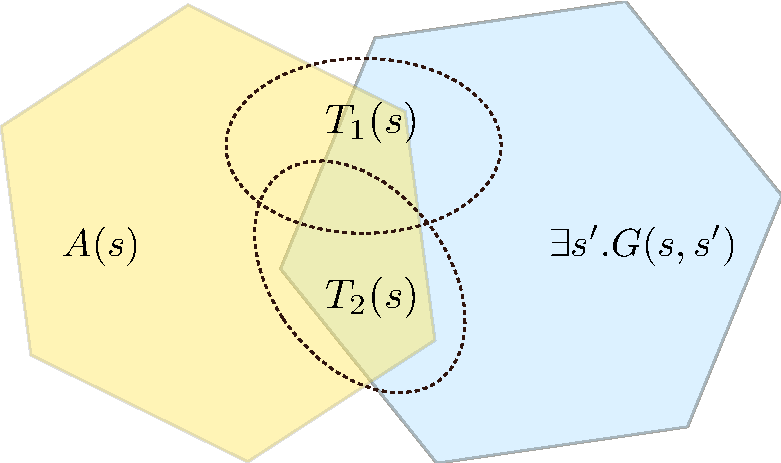
\includegraphics[width=3.5in]{aeval_invalid}
\caption{Region of validity computed for an example requiring \aeval to iterate two times.}
\label{fg:aeval}
\end{figure}

%\andreas{I believe the section can be a bit longer. I also think that the keyphrase ``region of validity'' needs to stand out more. Finally, a proof for Lemma 1, or at least an outline of it would be greatly appreciated.}

We rely on the already established algorithm to decide the validity of $\forall\exists$-formulas and extract Skolem functions, called \aeval~\cite{fedyukovich2015automated}.
It takes as input a formula of the form $\forall s \,.\,  A(s) \Rightarrow \exists s' . G(s,s')$,
where $A(s)$ has only existential quantifiers, and $G(s,s')$ is quantifier-free.
While deciding the validity, \aeval iteratively enumerates models of $A(s)$ and groups them into a set of partitions $\{T_i(s)\}$, such that each $T_i(s) \Rightarrow \exists s' . G (s, s')$.
We say that after $n$ iterations, \aeval establishes a formula $R_n(s) \eqdef \bigvee_{i=1}^n T_i(s)$ which is by definition an under-approximation of $\exists s' . G (s, s')$.
Figure~\ref{fg:aeval} shows a Venn diagram for an example of the (invalid) formula and $R_2 = T_1 \lor T_2$.
Because no model exists in $A(s) \land \neg{R_2(s)}$ then there does not exist a partition $T_3$, and \aeval terminates.
% \john {Because we are are already using $A$ and $G$ to represent meaningful formulas I suggest that we use different symbols here so it is not confusing. Especially because the symbols have different signatures in these locations.}

If after some $n$ iterations, it happens that $A(s) \Rightarrow R_n(s)$; then $\forall s \,.\,  A(s) \Rightarrow \exists s' . G(s,s')$ is valid, and \aeval generates a Skolem function as described in~\cite{katis2016synthesis}.
Intuitively, a Skolem function describes a connection between $s$ and $s'$; which, after conjoining to $A(s)$ and eliminating the existential quantifier in front of $G(s,s')$, makes the implication valid.

We say that $R_n(s)$ is a \emph{region of validity}, because $\forall s \,.\,  A(s) \land R_n(s) \Rightarrow \exists s' . G(s,s')$ is always valid by construction.
In this work, we are interested in the \emph{maximal} regions of validity, i.e., the ones produced by disjoining all partitions produced by \aeval before termination and by conjoining it further with $A(s)$.
Thus, throughout the paper, we assume that all regions of validity are maximal.
% \john{It is a bit strange how we alternate using formulas that have no free variables along with formulas whose free variables are meant to be implicitly existentially quantified. I think we should either stick with a notation or explicitly say that free variables are interpreted to be existentially quantified.}

\begin{lemma}
If formula $\forall s \,.\,  A(s) \Rightarrow \exists s' . G(s,s')$ is invalid, and $R_n(s)$ is the region of validity, then there is no other formula $S(s)$ such that $A(s) \land R_n(s) \Rightarrow S(s)$ and $\forall s \,.\,  S(s) \Rightarrow \exists s' . G(s,s')$.
\label{lem:subset}
\end{lemma}

\begin{proof}
Suppose that $S(s)$ exists.
Then $S(s) \land \neg{R_n(s)} \land A(s)$ is satisfiable, and its models are not contained in $R_n(s)$.
It contradicts our assumption that \aeval has terminated since otherwise it would proceed for generating $T_{n+1}(s)$ which in turn would enlarge the region of validity.
\end{proof}

\begin{corollary}
If formula $\forall s \,.\,  A(s) \Rightarrow \exists s' . G(s,s')$ is invalid, and $R_n(s)$ is the region of validity, then $A(s) \land R_n(s) \Leftrightarrow \exists s' . G(s,s')$.
\label{cor:intermediate}
\end{corollary}

\begin{proof}
($\Rightarrow$) is immediate from the definition of region of validity.
($\Leftarrow$).  Suppose towards contradiction that $s$ satisfies $\exists s' . G(s,s')$ but not $A(s) \land R_n(s)$.  If we define $S = s$, we violate Lemma~\ref{lem:subset}.
\end{proof} 

\iffalse
\begin{corollary}
If formula $\forall s \,.\,  A(s) \Rightarrow \exists s' . G(s,s')$ is invalid, and $A(s) \land R_n(s)$ is the region of validity, then 
 $\forall s \,.\, R_n(s) \Leftrightarrow (A(s) \Rightarrow \exists s' . G(s,s'))$ 
\label{cor:subset}
\end{corollary}

\begin{proof}
($\Rightarrow$) Given $s$, suppose $R_n(s)$ is true.  If $A(s)$ is false, then by Corollary~\ref{cor:intermediate},  $\exists s' . G(s,s')$ is false, so the implication holds.  Simlarly for $A(s)$ true.
($\Leftarrow$) Suppose $A(s) \Rightarrow \exists s' . G(s,s')$ is true.  Suppose $A(s)$ is false.  Then $G(s, s')$ might be true and $R_n(s)$ might be false, violating our equivalence.  Boo!
\end{proof}
\fi
